Исходно SSH model выглядит как
\begin{equation*}
	H = t_1 \sum_n \kb{n,B}{n,A} + t_2 \sum_n \kb{n+1, A}{n, B} + \hc
\end{equation*}
что в нашем случае переписывается в виде
\begin{equation*}
	H = \frac{\Omega_1}{2} \sum_p \kb{p,g}{p+1,e} + \frac{\Omega_2}{2} \sum_p \kb{p-1,e}{p,g} + \hc
\end{equation*}
где в случае с flashing коэффициенты становятся зависимыми от времени. Можно численно решить уравнение Линдблада для TLS в двух случаях
\begin{equation*}
	i \hbar \partial_t \rho = [H, \rho] + \mathcal{L}[\rho]
\end{equation*}


Таким образом принципиально делать лучи чередующимеся. Тут можно добавить картинку $\rho(t, k)$ (done) и схемы с ssh моделью и тем как лучи используем. 






\begin{figure}
    \centering
    \addletter{140}{a}
    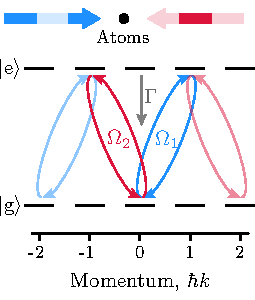
\includegraphics{fig-ai/ssh-scheme.pdf}
    \hfill
    \addletter{140}{b}
    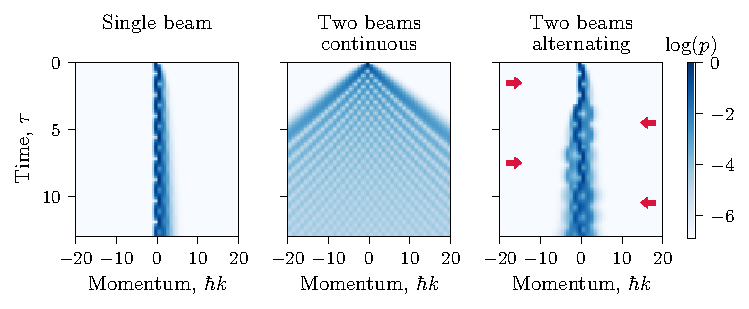
\includegraphics{fig-py/ssh-model.pdf}
    \caption{
        \textbf{Momentum-space dynamics in the SSH model}. 
        a) Atoms undergo momentum-changing transitions via couplings $\Omega_1$ and $\Omega_2$, realizing a SSH-like quantum walk.
        b) Momentum distributions over time for different beam configurations: single beam (left) shows small shift; two continuous beams (middle) result in fast spreading; alternating beams (right) suppress spread.
    }
    \label{fig:sshmodel}
\end{figure}









